\documentclass[9pt]{beamer}

/stock/16_git_repo/library/library.tex

\usetheme[compress]{Dresden2}
\usecolortheme{beaver}
\usecolortheme{seahorse}
%%\usecolortheme{spruce}
%
\setbeamertemplate{blocks}[rounded][shadow=true]
%\setbeamertemplate{navigation symbols}{} 
%%\setbeamercolor{block body alerted}{bg=red!30}
%%\setbeamercolor{block title alerted}{fg=white,bg=red}

\title[Elliptic Curve Cryptography]{The State of Elliptic Cryptography}
\author[G. Duvillié]{Guillerme Duvillié}
\institute{Université Montpellier 2}
%\logo{\includegraphics[scale=0.03]{um2.png}}

\AtBeginSection[]{
    \begin{frame}{Plan}
        \tableofcontents[currentsection]
    \end{frame}
}

\floatname{algorithm}{Procedure}
\renewcommand{\algorithmicrequire}{\textbf{Input:}}
\renewcommand{\algorithmicensure}{\textbf{Output:}}

\begin{document}

\begin{frame}
    \titlepage
\end{frame}

\addtocounter{framenumber}{-1}
\addtobeamertemplate{footline}{\insertframenumber/\inserttotalframenumber}

\section{Introduction}

\subsection*{A}

% {{{ Historique
\begin{frame}
    \frametitle{Historique}
    \vfill
    \begin{itemize}
        \item[1874 $\bullet$] Introduction du problème de factorisation par William Stanley
            Jevon
            \vfill
            \pause
        \item[1976 $\bullet$] Échange de clé de Whitfielf Diffie et Martin Edward Hellman
            \vfill
            \pause
        \item[1977 $\bullet$] RSA par Ron Rivest, Adi Shamir et Leonard Adleman
            \vfill
            \pause
        \item[1985 $\bullet$] Taher ElGamal introduit un nouveau cryptosystème basé sur DLP
            \vfill
            \pause
        \item[1985 $\bullet$] Neal Koblitz et Victor Saul Miller introduisent la
            cryptographie sur courbe elliptique
            \vfill
    \end{itemize}
\end{frame}
% }}}

% {{{ Comparatif
\begin{frame}
    \frametitle{La cryptographie sur courbes elliptiques}
    \begin{columns}[tb]
        \begin{column}{0.35\linewidth}
            \vfill
            \begin{figure}
                \begin{center}
                    \includegraphics[scale=0.18]{ecc.png}
                \end{center}
                \caption{Une courbe elliptique}
            \end{figure}
        \end{column}
        \begin{column}{0.6\linewidth}
            \begin{itemize}
                \item[\textcolor{green}{+}] Pas d'algorithmes sous exponentiels
                    \vfill
                    \pause
                \item[\textcolor{green}{+}] Groupe de plus petite taille
                    \vfill
                    \pause
                \item[\textcolor{green}{+}] Une clé plus petite
                    \vfill
                    \pause
                \item[\textcolor{green}{+}] Implémentations plus rapide
                    \vfill
                    \pause
                \item[\textcolor{red}{-}] Théorie un peu plus compliquée
            \end{itemize}
        \end{column}
    \end{columns}
\end{frame}
% }}}

\section{Théorie}

\subsection*{b}

\begin{frame}
    \frametitle{Caractéristique d'un corps}
    \begin{df}[Caractéristique d'un corps]
        Soient un corps $K = (K, +, \times)$, $0$ le neutre pour l'addition et $1$ le neutre pour la
        multiplication, la caractéristique de $K$ est la plus petit entier $n$ tel que :
        \[
            \begin{array}{ccc}
                \underbrace{1 + \dots + 1} & = & 0 \\
                n \mbox{ fois} & & \\
            \end{array}
        \]
        On le note $char(n)$.
    \end{df}
    \begin{exampleblock}{Exemple}
        Soit $\mathbb{F}_7 = \mathbb{Z}/7\mathbb{Z}$ : 
        \[ char(\mathbb{F}_7) = 7 \]
    \end{exampleblock}
\end{frame}

\begin{frame}
    \frametitle{Courbes elliptique sur $K$ avec $char(K) \neq 2,3$}
    \begin{df}
        Soit un corps $K$ tel que $char(K) \neq 2, 3$ et soit un polynome cubique de la forme $x^3 +
        cx + d$ n'admettant aucune racines multiples. Une courbe elliptique $E$ sur $K$ est un
        ensemble de points $(x,y) \in K^2$ vérifiant l'équation :
        \[
            y^2 = x^3 + cx + d
        \]
        avec $c, d \in K$, auquel on ajoute un point $\mathcal{O}$ à l'infini.
    \end{df}

    \begin{thrm}
        Soit $p(x) = ax^3 + bx^2 + cx + d$, un polynome dont les coefficients sont à valeur dans $K$, $p$ n'admet pas de
        racines multiples ssi : \[
            \Delta =  b^2c^2 - 4ac^3 - 4b^3d - 27a^2d^2 + 18abcd \neq 0
        \]
    \end{thrm}
    \begin{corol}
        $p = x^3 + cx + d$ n'admet pas de racines multiples ssi $4c^3 + 27d^2 \neq 0$
    \end{corol}
\end{frame}

\begin{frame}
    \frametitle{La courbe elliptique $y^2 = x^3 + x$ sur $\mathbb{Q}$}
    \begin{figure}
        \includegraphics[scale=0.5]{ecc.png}
    \end{figure}
\end{frame}

\begin{frame}
    \frametitle{La courbe elliptique $y^2 = x^3 + x$ sur $\mathbb{Z}/7\mathbb{Z}$}
    \begin{figure}
        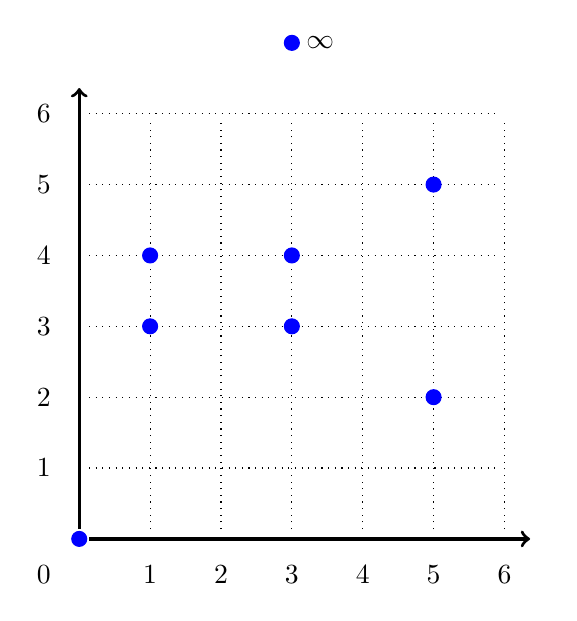
\begin{tikzpicture}[scale=0.9]
            \node (0y) at (0, 0) {};
            \node (yy) at (0, 6.5) {};
            \node (0x) at (0, 0) {};
            \node (xx) at (6.5, 0) {};

            \node (0lab) at (-0.5, -0.5) {$0$};
            \node (inf) at (3.4, 7) {$\infty$};

            \draw[->, very thick] (0y) to (yy);
            \draw[->, very thick] (0x) to (xx);

            \foreach \x in {1,...,6}{
                \node (y\x) at (\x, 0) {};
                \node (yy\x) at (\x, 6) {};
                \node (xlab\x) at (\x, -0.5) {$\x$};
                \node (x\x) at (0, \x) {};
                \node (xx\x) at (6, \x) {};
                \node (ylab\x) at (-0.5, \x) {$\x$};

                \draw[-, dotted] (y\x) to (yy\x);
                \draw[-, dotted] (x\x) to (xx\x);
            }

            \filldraw[blue] (0,0) circle (3pt)
                            (1,3) circle (3pt)
                            (1,4) circle (3pt)
                            (3,3) circle (3pt)
                            (3,4) circle (3pt)
                            (5,5) circle (3pt)
                            (3,7) circle (3pt)
                            (5,2) circle (3pt);
        \end{tikzpicture}
    \end{figure}
\end{frame}

\begin{frame}
    \frametitle{Courbes elliptique sur $K$ avec $char(K) = 2$}
    \begin{df}
        Soit un corps $K$ tel que $char(K) = 2$. Une courbe elliptique $E$ sur $K$ est un
        ensemble de points $(x,y) \in K^2$ vérifiant satisfaisant une équation du type soit:
        \[
            y^2 + ey = x^3 + cx + d
        \]
        soit : 
        \[
            y2 + xy = x^3 + cx + d
        \]
        avec $c, d, e \in K$, auquel on ajoute un point $\mathcal{O}$ à l'infini.
    \end{df}

    \begin{rmq}
        Dans ce cas, le polynome de droite peut avoir des racines multiples.
    \end{rmq}
\end{frame}

\begin{frame}
    \frametitle{La courbe elliptique $y^2 + y= x^3$ sur $\mathbb{Q}$}
    \begin{figure}
        \includegraphics[scale=0.5]{ecc2.png}
    \end{figure}
\end{frame}

\begin{frame}
    \frametitle{La courbe elliptique $y^2 + y = x^3$ sur $\mathbb{Z}/2\mathbb{Z}$}
    \begin{figure}
        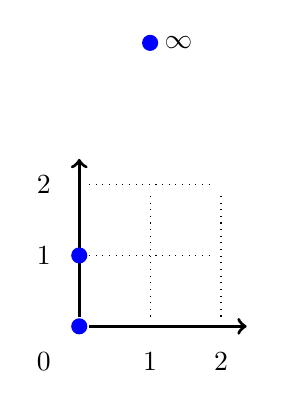
\begin{tikzpicture}[scale=0.9]
            \node (0y) at (0, 0) {};
            \node (yy) at (0, 2.5) {};
            \node (0x) at (0, 0) {};
            \node (xx) at (2.5, 0) {};

            \node (0lab) at (-0.5, -0.5) {$0$};
            \node (inf) at (1.4, 4) {$\infty$};

            \draw[->, very thick] (0y) to (yy);
            \draw[->, very thick] (0x) to (xx);

            \foreach \x in {1,...,2}{
                \node (y\x) at (\x, 0) {};
                \node (yy\x) at (\x, 2) {};
                \node (xlab\x) at (\x, -0.5) {$\x$};
                \node (x\x) at (0, \x) {};
                \node (xx\x) at (2, \x) {};
                \node (ylab\x) at (-0.5, \x) {$\x$};

                \draw[-, dotted] (y\x) to (yy\x);
                \draw[-, dotted] (x\x) to (xx\x);
            }

            \filldraw[blue] (0,0) circle (3pt)
                            (1,4) circle (3pt)
                            (0,1) circle (3pt);
        \end{tikzpicture}
    \end{figure}
\end{frame}

\begin{frame}
    \frametitle{Courbes elliptique sur $K$ avec $char(K) = 3$}
    \begin{df}
        Soit un corps $K$ tel que $char(K) = 3$. Une courbe elliptique $E$ sur $K$ est un
        ensemble de points $(x,y) \in K^2$ vérifiant satisfaisant une équation du type :
        \[
            y^2 = x^3 + bx^2 + cx + d
        \]
        avec $c, d, e \in K$, auquel on ajoute un point $\mathcal{O}$ à l'infini.
    \end{df}

    \begin{rmq}
        Dans ce cas, le polynome de droite ne peut avoir des racines multiples.
    \end{rmq}

    \begin{rmq}
        Le polynome $p(x) = x^3 + bx^2 + cx + d$ n'a pas de racines multiples ssi : \[
            b^2c^2 - 4 c^3 - 4b^3d - 27d^2 + 18 bcd \neq 0
        \]
    \end{rmq}
\end{frame}

\begin{frame}
    \frametitle{La courbe elliptique $y^2 = x^3 + 6y^2 + 5x + 1$ sur $\mathbb{Q}$}
    \begin{figure}
        \includegraphics[scale=0.5]{ecc3.png}
    \end{figure}
\end{frame}

\begin{frame}
    \frametitle{La courbe elliptique $y^2 = x^3 + 6y^2 + 5x + 1$ sur $\mathbb{Z}/3\mathbb{Z}$}
    \begin{figure}
        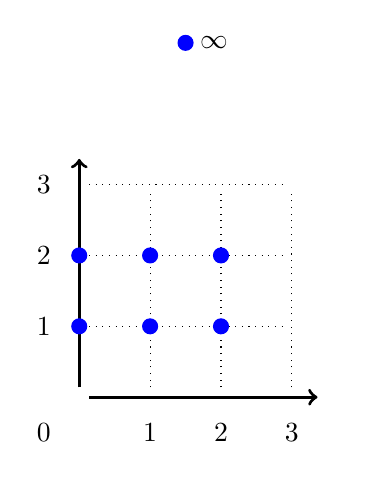
\begin{tikzpicture}[scale=0.9]
            \node (0y) at (0, 0) {};
            \node (yy) at (0, 3.5) {};
            \node (0x) at (0, 0) {};
            \node (xx) at (3.5, 0) {};

            \node (0lab) at (-0.5, -0.5) {$0$};
            \node (inf) at (1.9, 5) {$\infty$};

            \draw[->, very thick] (0y) to (yy);
            \draw[->, very thick] (0x) to (xx);

            \foreach \x in {1,...,3}{
                \node (y\x) at (\x, 0) {};
                \node (yy\x) at (\x, 3) {};
                \node (xlab\x) at (\x, -0.5) {$\x$};
                \node (x\x) at (0, \x) {};
                \node (xx\x) at (3, \x) {};
                \node (ylab\x) at (-0.5, \x) {$\x$};

                \draw[-, dotted] (y\x) to (yy\x);
                \draw[-, dotted] (x\x) to (xx\x);
            }

            \filldraw[blue] (0,1) circle (3pt)
                            (0,2) circle (3pt)
                            (1,1) circle (3pt)
                            (1,2) circle (3pt)
                            (2,1) circle (3pt)
                            (2,2) circle (3pt)
                            (1.5,5) circle (3pt);
        \end{tikzpicture}
    \end{figure}
\end{frame}

\begin{frame}
    \frametitle{Propriétés}
    \begin{thrm}
        $E$ est un groupe additif abélien, avec le point $\mathcal{O}$ servant de neutre.
    \end{thrm}

    \begin{df}
        Si $char(K) \neq 2,3$, la loi d'addition est définie ainsi : soit $P,Q \in E$, $P = (x_1,
        y_1),\ Q = (x_2, y_2)$ alors $-P = (x_1, y_1)$ $P + Q = (x_3, y_3)$ avec : \[
            \begin{array}{rcl}
                x_3 & = & \lambda^2 - x_1 - x_2 \\
                y_3 & = & \lambda(x_1 - x_3) - y_1
            \end{array}
        \]
        avec : \[
            y = \left \lbrace \begin{array}{rcl}
                \displaystyle \frac{y_2 - y_1}{x_2 - x_1} & \mbox{ si } & P \neq Q \\
                \displaystyle \frac{3x_1^2 + a}{2y_1} & \mbox{ si } & P = Q \\
                \end{array} \right.
            \]
    \end{df}
\end{frame}

\begin{frame}
    \frametitle{Exemple sur $\mathbb{R}$, $E : y^2 = x^3 - 5x + 4$}
    \begin{figure}
        \includegraphics[scale=0.5]{ecc41.png}
    \end{figure}
\end{frame}

\begin{frame}
    \frametitle{Exemple sur $\mathbb{R}$, $E : y^2 = x^3 - 5x + 4$}
    \begin{figure}
        \includegraphics[scale=0.5]{ecc42.png}
    \end{figure}
\end{frame}

\begin{frame}
    \frametitle{Exemple sur $\mathbb{R}$, $E : y^2 = x^3 - 5x + 4$}
    \begin{figure}
        \includegraphics[scale=0.5]{ecc43.png}
    \end{figure}
\end{frame}

\begin{frame}
    \frametitle{Exemple sur $\mathbb{R}$, $E : y^2 = x^3 - 5x + 4$}
    \begin{figure}
        \includegraphics[scale=0.5]{ecc44.png}
    \end{figure}
\end{frame}

\begin{frame}
    \frametitle{Rapport}
    \dfpbi{\dlp}{Un groupe fini et cyclique $G$, $g$ et $h \in G$}{Trouver $a$ tel que $g^a = h$}
\end{frame}

\section{Applications aux cryptosystèmes}



\end{document}
